\section{ASCbase::hbond\_\-surface\_\-t Class Reference}
\label{classASCbase_1_1hbond__surface__t}\index{ASCbase::hbond_surface_t@{ASCbase::hbond\_\-surface\_\-t}}
{\tt \#include $<$Hbond\-Surfaces.H$>$}

Inheritance diagram for ASCbase::hbond\_\-surface\_\-t::\begin{figure}[H]
\begin{center}
\leavevmode
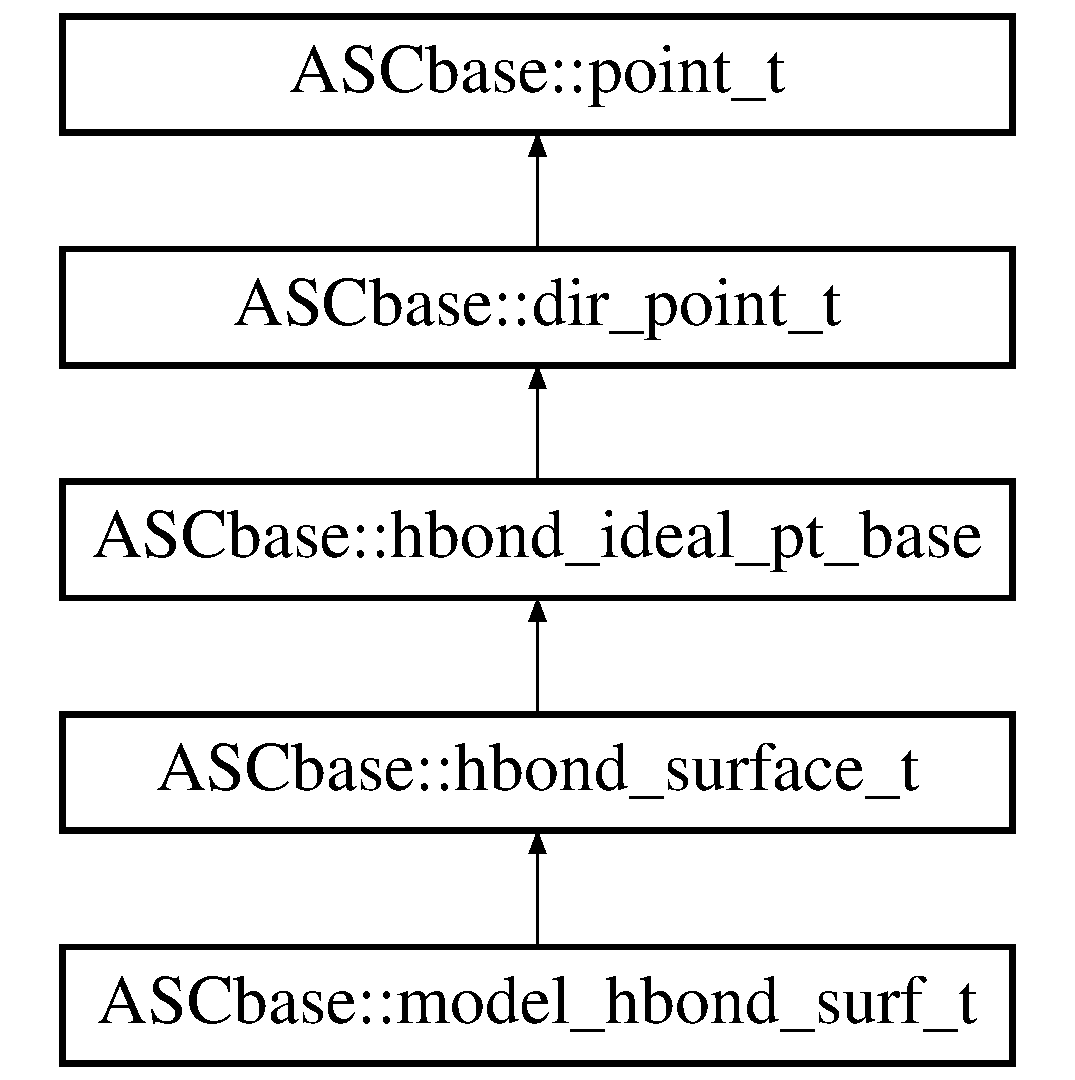
\includegraphics[height=5cm]{classASCbase_1_1hbond__surface__t}
\end{center}
\end{figure}
\subsection*{Public Member Functions}
\begin{CompactItemize}
\item 
\bf{hbond\_\-surface\_\-t} (const atom\_\-vci hbond\_\-atom, const atom\_\-vci C\_\-nbr\_\-atom, const atom\_\-vci second\_\-nbr\_\-atom, \bf{Bounding\-Volume} \&site\_\-vol, const int cap\_\-number, const bool include\_\-metals=false, const alloc\_\-t a=ALLOC\_\-POSITION)\label{classASCbase_1_1hbond__surface__t_9e357e26963a25f5d34f8ead0e7154b8}

\begin{CompactList}\small\item\em Constructor to create the representation. \item\end{CompactList}\item 
\bf{hbond\_\-surface\_\-t} (const std::string \&data\_\-line, \bf{PDBBase} \&prot\_\-atoms)\label{classASCbase_1_1hbond__surface__t_a072af1ca67675f348af7ae0f6a9941b}

\begin{CompactList}\small\item\em Constructor for an existing surface (typically read from file). \item\end{CompactList}\item 
\textbf{hbond\_\-surface\_\-t} (const \bf{hbond\_\-surface\_\-t} \&src)\label{classASCbase_1_1hbond__surface__t_e1e229896cc8285447726191d4c8e5c2}

\item 
const \bf{hbond\_\-surface\_\-t} \& \textbf{operator=} (const \bf{hbond\_\-surface\_\-t} \&src)\label{classASCbase_1_1hbond__surface__t_c825922a0e490482d7f5362d2554beaf}

\item 
bool \textbf{closest\_\-point} (const my\_\-float\_\-t $\ast$pt, my\_\-float\_\-t $\ast$closest\_\-pt, const my\_\-float\_\-t tol=1.0)\label{classASCbase_1_1hbond__surface__t_828b634e714761ec0282112bab50d6f6}

\item 
const my\_\-float\_\-t $\ast$ \textbf{ideal\_\-dir} () const \label{classASCbase_1_1hbond__surface__t_64bcfe8ebae6a5a406fa880eabe4c0b6}

\item 
void \textbf{transform} (const my\_\-float\_\-t $\ast$R, const my\_\-float\_\-t $\ast$T)\label{classASCbase_1_1hbond__surface__t_81063d19a3920c08e846d70928f6c594}

\item 
void \textbf{inverse\_\-transform} (const my\_\-float\_\-t $\ast$R, const my\_\-float\_\-t $\ast$T)\label{classASCbase_1_1hbond__surface__t_203a7593526f7b8d8a20cb664406d6a3}

\item 
void \textbf{revert} ()\label{classASCbase_1_1hbond__surface__t_e65041fc31bbbaae6922364cfe78ae54}

\end{CompactItemize}
\subsection*{Private Member Functions}
\begin{CompactItemize}
\item 
void \textbf{do\_\-copy} (const \bf{hbond\_\-surface\_\-t} \&src)\label{classASCbase_1_1hbond__surface__t_e9299a1f7a8dbf67c3136863dd2df237}

\end{CompactItemize}
\subsection*{Private Attributes}
\begin{CompactItemize}
\item 
geometry::sphere\_\-t \textbf{A\_\-surf}\label{classASCbase_1_1hbond__surface__t_95bfd3372bb83fadd0b1708da01dec8d}

\item 
\bf{geometry::plane\_\-t} \textbf{A\_\-cut\_\-plane}\label{classASCbase_1_1hbond__surface__t_397632033debf716dbcc7fc8ef81fb61}

\item 
my\_\-float\_\-t \bf{A\_\-cap\_\-plane\_\-rad}\label{classASCbase_1_1hbond__surface__t_83046f180c928461d3f67c4b3b81554c}

\begin{CompactList}\small\item\em Radius of cap restricted to cutting plane. \item\end{CompactList}\item 
std::vector$<$ \bf{geometry::i\-Circle} $>$ \textbf{A\_\-circles}\label{classASCbase_1_1hbond__surface__t_f0161567ebb1e37b69510969d76ddb86}

\end{CompactItemize}
\subsection*{Static Private Attributes}
\begin{CompactItemize}
\item 
static const my\_\-float\_\-t \bf{SURF\_\-SPHERE\_\-RAD} = 3.0\label{classASCbase_1_1hbond__surface__t_5779dc1ca7f6d66ef343d01ba14978b8}

\begin{CompactList}\small\item\em Radius of sphere used to define the cap. \item\end{CompactList}\end{CompactItemize}


\subsection{Detailed Description}
I am currently in a bind and to get this working quickly, I am abusing the format to handle metals as well. In the case of metals we do NOT have neighbor atom or an initial cap cutting plane (metals are modeled as not having a prefered direction). However, we do desire to keep the method transformation invariant; to do this we put the closest atom to the metal as the C\_\-nbr\_\-atom and the 2nd closest as the 2nd nbr atom (this is confusing but quick \& dirty). 



The documentation for this class was generated from the following files:\begin{CompactItemize}
\item 
Hbond\-Surfaces.H\item 
Hbond\-Surfaces.C\end{CompactItemize}
